\documentclass[12pt]{article}

\usepackage{amsmath}
\usepackage{enumitem}
\usepackage[margin=1.5in]{geometry}
\usepackage{hyperref}
\usepackage[utf8]{inputenc}
\usepackage{graphicx}
\usepackage{rotating}

\title{Not exactly the Internet of Things for Outdoor Lighting: Requirements Document}
\author{Oregon State University CS Senior Capstone Group 22\\Malcolm Diller, Sean Rettig, Evan Steele\\Client: Victor Hsu}
\begin{document} 

\maketitle

\pagebreak

\section{Team Name}

Cupcake Warriors

\section{Team Members}

\begin{tabular}{ l l } 
    Malcolm Diller & dillerm@oregonstate.edu\\ 
    Sean Rettig & rettigs@oregonstate.edu\\
    Evan Steele & steelee@oregonstate.edu\\ \end{tabular}

\section{Client}

Victor Hsu\\
Oregon State University\\
Phone: 541-737-4398\\
Email: hsuv@onid.orst.edu

\section{Problem Statement}

Outdoor lighting seems like a simple problem to solve, but the solutions on the
market today are less than ideal.  The standard transformer/timer combos
available in the big box stores are rudimentary and clunky at best (constantly
needing to be adjusted for the changing sunset and sunrise times), but are
reasonably priced. The new-generation smart apps for home automation are
flexible and fancier, but are quite spendy and lock you into a specific
protocol.  So why not use an open platform running on commodity hardware?  Easy
to use, reasonably priced, and highly customizable--that is our goal.

\section{Project Description}

Our system will consist of a wireless network of tiny “client” computers that
each control up to 4 sets of lights and are controlled by a central "server"
computer, which will automatically send out commands to the clients when it's
time to turn on or off.  The central node will run a control program that can
be easily accessed via a touch screen, a web browser, or a mobile device, where
the user can locally or remotely control each light individually.  Want your
lights to turn on at sunset and then dim gradually as the sun rises?  Simple.
Want your lights to flash when you're throwing a party?  Just press a button.
The control interface will allow users to easily set "rules" for what their
lights do and when, depending on the time of day, the sun/moon position, and
potentially even triggers such as weather conditions or calendar dates.  This
system will be easily extensible to potentially control other devices as well,
such as garage doors, sound systems, and more.

\section{Design}

Specifically, we plan to use a Raspberry Pi running Linux as the central server
computer.  The Raspberry Pi will run a web server program that will allow
nearby devices (such as laptops, phones, or tablets) to control it over a
wireless network, or if connected to the home's internet connection, from
practically anywhere in the world.  The Pi will also have a small touchscreen
connected to it with the website open in a browser, so the user has a dedicated
interface for the device.  The Pi will connect wirelessly to small wifi-enabled
microcontrollers placed throughout the home, each of which are connected to up
to 4 relays to control 4 sets of lights.

\section{Requirements}

\subsection{Critical Requirements}

The following requirements are critical to the basic functionality of the
system and must be functional prior to the expo in spring term.

\begin{enumerate}
    \item Device control
        \begin{enumerate}
            \item Server is loaded with firmware and is able to boot
            \item Server is able to start the server control program automatically when powered on
            \item Clients are loaded with firmware and are able to boot
            \item Clients are able to start the client control program automatically when powered on
            \item Client control program is able to automatically discover relays/lights that are connected to it
            \item Client control program can control the relays to power the lights on/off individually
            \item Lights can be toggled over a user-specified period of time, e.g. a light can gradually turn on and grow brighter over the course of 30 seconds
            \item Clients can be paired with a server by pressing a button on each device at the same time, allowing multiple servers to be used in close proximity
            \item Clients are able to communicate to the server which lights are available for control
            \item Server is able to send light toggle instructions wirelessly to clients
            \item Clients are able to read light toggle instructions wirelessly from the server
            \item Clients are able to perform light toggle instructions received from the server
        \end{enumerate}

    \item User interface
        \begin{enumerate}
            \item Main control program on server serves a web site with a control interface for the user
            \item The web interface is accessible via the system's built-in touchscreen
            \item The web interface is accessible to other devices like laptops and phones via a local wireless network
            \item The web interface displays a list of connected clients
            \item The web interface allows users to give each client a "nickname" for easy identification
            \item The web interface displays a list of connected lights
            \item The web interface allows users to give each light a "nickname" for easy identification
            \item The web interface contains buttons for each light that can be used to control lights individually
            \item The web interface contains the ability to put lights into "groups" that can be controlled together all at once
            \item The web interface displays a list of light groups
            \item The web interface allows users to give each light group a "nickname" for easy identification
            \item Groups can also be nested into other groups to create hierarchies of lights
            \item The web interface provides the user with options to toggle lights/groups based on rules, as described in the below "Rules" section
        \end{enumerate}

    \item Rules
        \begin{enumerate}
            \item Lights can be toggled manually, overriding any rules
            \item Lights can be toggled based on time of day (e.g. "turn on at 8pm and turn off at 6am")
            \item Lights can be toggled based on day of week (e.g. "turn on during Wednesdays")
            \item Lights can be toggled based on day of month (e.g. "turn on every 1st of the month")
            \item Lights can be toggled based on day of year (e.g. "turn on every January 1st")
            \item Lights can be toggled based on specific dates (e.g. "turn on from Dec. 24th at 2am to Dec 27th at 8pm")
            \item Lights can be toggled based on sunrise/sunset times
            \item Multiple rules can be applied to a single light/group using an AND/OR system to combine the rules (e.g. "turn on between 8pm and 6am AND turn on on Wednesday" will turn the lights on between 8pm and 6am on Wednesdays, and will be off the rest of the time, whereas using an OR instead of an AND would cause the lights to be on every day from 8pm to 6am and also on all day during Wednesday)
            \item Lights can be toggled based on the toggle state of its parent group (e.g. by default, a light will turn on if its parent group turns on, but it can also be set to turn off if the parent group turns on)
            \item Rules can be set to toggle early/late by a constant or random period of time
            \item Lights within a group can be set to toggle early/late by a random period of time so that they toggle in a staggered fashion
        \end{enumerate}
\end{enumerate}

\subsection{Stretch Goals}

The following requirements are optional; they are not critical to the basic
functionality of the system and may be implemented only if time permits.

\begin{enumerate}[resume]
    \item Device control
        \begin{enumerate}
            \item System also controls devices other than lights
                \begin{enumerate}
                    \item Garage door openers
                    \item Music players
                    \item Holiday decorations
                    \item Sprinkler systems
                \end{enumerate}
        \end{enumerate}
    \item User interface
        \begin{enumerate}
            \item The web interface is accessible over the Internet
                \begin{enumerate}
                    \item The web interface is accessible only to the homeowner or other authorized individuals
                    \item The web interface is hosted on a remote server for high availablity and the lack of need for the user to perform port forwarding on their router
                \end{enumerate}
        \end{enumerate}
    \item Rules
        \begin{enumerate}
            \item Lights can be toggled based on weather conditions (would require Internet connection or light/moisture sensors)
            \item Lights can be toggled based on a schedule in the user's calendar, e.g. Google calendar (would require Internet connection)
            \item Lights can be toggled based on moon position or other celestial data
            \item Lights can be toggled based on input from attached sensors
                \begin{enumerate}
                    \item Motion sensors
                    \item Light sensors
                    \item Moisture sensors
                    \item Sound sensors
                \end{enumerate}
        \end{enumerate}
\end{enumerate}

\section{Preliminary Timetable}

By the end of fall term, we plan to have a working proof-of-concept, using the
Raspberry Pi and a basic control program to toggle lights on and off.  By the
end of winter term, we plan to have all required features at least partially
implemented, at which our project enters the beta phase.  As we finish up by
ironing out bugs and perhaps completing stretch goals, we will release version
1.0 prior to the expo.

\subsection{Gantt Chart}
Gantt chart available at our project SharePoint website: \url{https://oregonstateuniversity-my.sharepoint.com/personal/rettigs_oregonstate_edu/capstone22_project/_layouts/15/start.aspx#/Lists/Tasks/gantt.aspx}
\begin{sidewaysfigure}
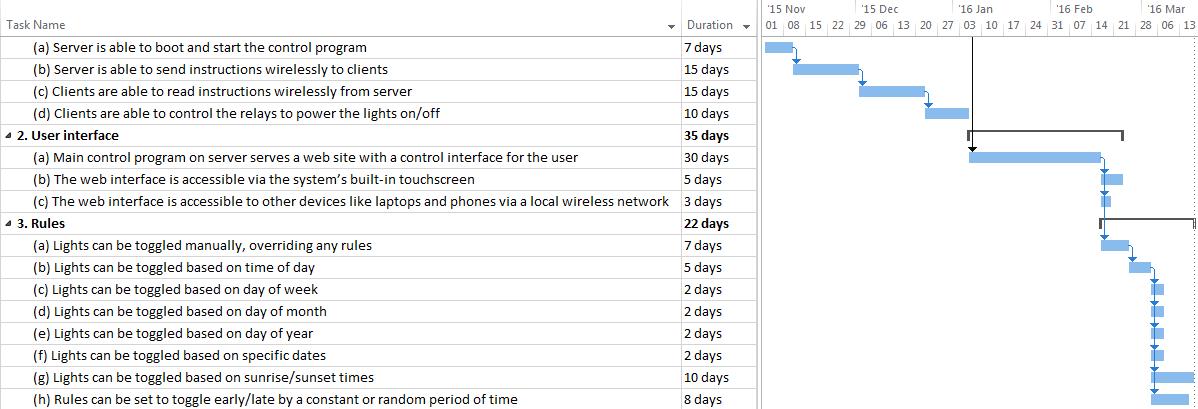
\includegraphics[width=1.1\textwidth]{gantt.png}
\end{sidewaysfigure}

\pagebreak

\section{Signatures}

\begin{tabular}{l l l l} Malcolm Diller & \underline{\hspace{6cm}} & Date
\underline{\hspace{2cm}}\\ Sean Rettig & \underline{\hspace{6cm}} & Date
\underline{\hspace{2cm}}\\ Evan Steele & \underline{\hspace{6cm}} & Date
\underline{\hspace{2cm}}\\ Victor Hsu & \underline{\hspace{6cm}} & Date
\underline{\hspace{2cm}} \end{tabular}
    
\end{document}
